\documentclass{article}
\usepackage[utf8]{inputenc}
\usepackage{cancel}
\usepackage{amsthm,amssymb,amsmath}
\usepackage{mathtools}
\usepackage{tikz}
% in preamble
\usepackage{movie15}
% in documenet
\usepackage{fouriernc}
\usepackage{tkz-euclide}
\usetikzlibrary{calc, backgrounds}
\usepackage{tikz-3dplot}
\usetikzlibrary{positioning}
\usepackage{parskip}
\usepackage{float}
\tdplotsetmaincoords{70}{0}%
\newtheorem{theorem}{Theorem}[section]
\newtheorem{corollary}{Corollary}[theorem]
\newtheorem{lemma}[theorem]{Lemma}
\setlength{\parskip}{1em}
\newcommand{\NN}{\mathbb{N}}
\newcommand{\ZZ}{\mathbb{Z}}
\newcommand{\RR}{\mathbb{R}}
\newcommand{\QQ}{\mathbb{Q}}
\newcommand{\CC}{\mathbb{C}}
\tdplotsetmaincoords{60}{110}
\def\r{{2*sqrt(3)}}
\title{MAT 4800 Homework \# 5 }
\author{Noah Reef }
\date{Spring 2023}

\usepackage{natbib}
\usepackage{graphicx}

\begin{document}
\maketitle

\section*{Problem \#1}
Here we are asked to find the ``largest circular cylinder that can be inscribed in a sphere of a given radius" to do this we first note that the volume of cylinder is denoted as,

\begin{equation*}
    V_{c} = \pi r_c^2h_c
\end{equation*}
where $r_c$ is the radius of the cylinder and $h_c$ is the height of the cylinder. Now supposing that circular cylinder is inscribed in a sphere with fixed radius $r_0$, our goal is now to,
\begin{align*}
    \max{V_c} &=\pi r_c^2 h_c\\ \\
    \text{subject to:}\\
    &r_c^2 + \left(\frac{h_c}{2}\right)^2 = r_0^2 
\end{align*}


\begin{figure}[H]
    \centering
    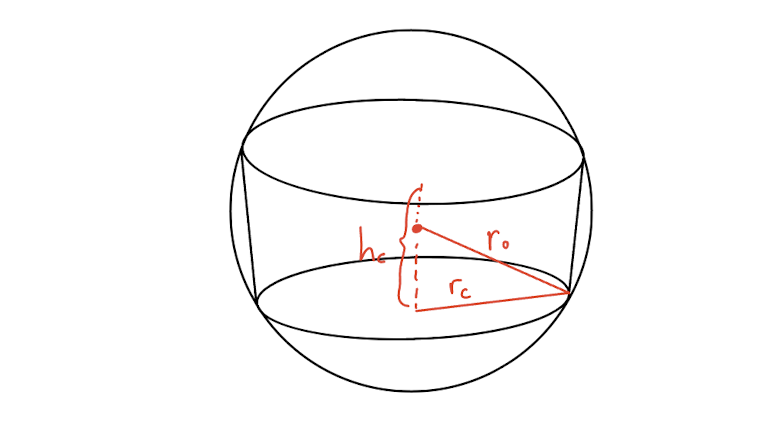
\includegraphics[scale=0.6]{Screenshot 2023-03-08 at 5.22.19 PM.png}
    \caption{Cylinder Inscribed in Sphere with fixed radius $r_0$}
    \label{fig:my_label}
\end{figure}

Note that we can rewrite the above constraint as,

\begin{equation*}
    \frac{2}{3}\left(\frac{r_c^2}{2}\right) + \frac{1}{3}\left(\frac{h_c}{2}\right)^2 = \frac{1}{3}r_0^2 
\end{equation*}

then by the A-G inequality we get,

\begin{equation*}
   \left(\left(\frac{r_c^2}{2}\right)^{2/3} \left(\frac{h_c}{2}\right)^{2/3}\right) \leq \frac{2}{3}\left(\frac{r_c^2}{2}\right) + \frac{1}{3}\left(\frac{h_c}{2}\right)^2 = \frac{1}{3}r_0^2 
\end{equation*}
with,

\begin{equation*}
    \left(\left(\frac{r_c^2}{2}\right)^{2/3} \left(\frac{h_c}{2}\right)^{2/3}\right) = \left( \frac{1}{4}r_c^2h_c\right)^{2/3} = \left( \frac{1}{4\pi}V_c\right)^{2/3} \leq \frac{1}{3}r_0^2
\end{equation*}

or,

\begin{equation*}
    V_c \leq \frac{4\pi r_0^3}{3\sqrt{3}}
\end{equation*}

note that we attain equality when,

\begin{equation*}
    \frac{r_c^2}{2} = \frac{h_c^2}{4}
\end{equation*}

and get,

\begin{equation*}
    r_c = \sqrt{\frac{2}{3}}r_0
\end{equation*}

and,

\begin{equation*}
    h_c = \frac{2}{\sqrt{3}}r_0
\end{equation*}

to get,

\begin{equation*}
    V_c = \frac{4\pi r_0^3}{3\sqrt{3}}
\end{equation*}
\section*{Problem \#2}
Here we will solve again the problem above using the standard calculus approach. First note the formula above for the volume a cylinder inscribed in a sphere with a fixed radius as,

\begin{equation*}
    V_c = 2\pi r_c^2\sqrt{(r_0^2 - r_c^2)}
\end{equation*}

next we take the derivative as,

\begin{equation*}
    \frac{d}{dr_c}V_c = 4\pi r_c\sqrt{(r_0^2-r_c^2)} -2\pi r_c^3(r_0^2-r_c^2)^{-1/2}
\end{equation*}

and setting it equal to $0$,

\begin{equation*}
    4\pi r_c\sqrt{(r_0^2-r_c^2)} -2\pi r_c^3(r_0^2-r_c^2)^{-1/2} = 0
\end{equation*}

\begin{equation*}
    2(r_0^2-r_c^2) = r_c^2
\end{equation*}

\begin{equation*}
    r_c = \sqrt{\frac{2}{3}}r_0
\end{equation*}

and plugging into $h_c$ to find,

\begin{equation*}
    h_c = \frac{2}{\sqrt{3}}r_0
\end{equation*}

we also find the volume of the inscribed circular cylinder as,

\begin{equation*}
    V_c = \frac{4\pi r_0^3}{3\sqrt{3}}
\end{equation*}
which is the same as above in \textbf{Problem \#1}

\section*{Problem \#3}

\begin{figure}[H]
    \centering
    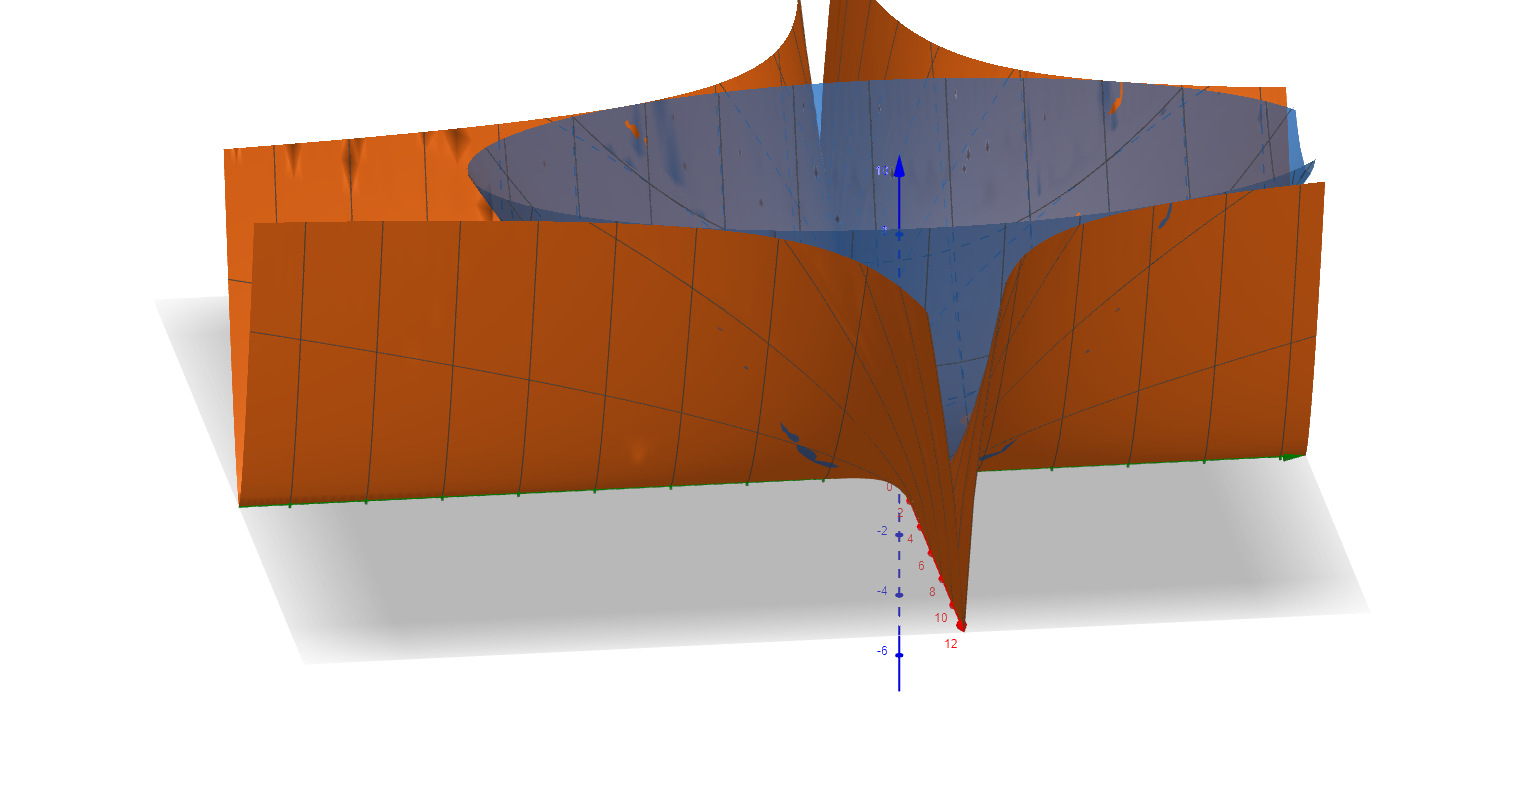
\includegraphics[scale=0.2]{fig1.png}
    \caption{Plot of Summation (Blue) and Product (Orange)}
    \label{fig:my_label}
\end{figure}

Here we see that the product is below the summation, which agrees with our AG inequality.

\section*{Problem \#4}
Here we want to find the smallest radius $r$ such that a circular cylinder of volume $8$ cubic units can be inscribed in a a sphere of radius $r$, that is we want to do the following,

\begin{align*}
    \min{r^2} &= r_c^2 + \left(\frac{h_c}{2}\right)^2\\ \\
    \text{subject to:}\\
    &\pi r_c^2h_c = 8\\
\end{align*}

note that we can write the following,

\begin{equation*}
    \frac{2}{3}\left(\frac{r_c^2}{2}\right) + \frac{1}{3}\left(\frac{h_c}{2}\right)^2 = \frac{1}{3}r^2 
\end{equation*}

then by the A-G inequality we get,

\begin{equation*}
   \left(\left(\frac{r_c^2}{2}\right)^{2/3} \left(\frac{h_c}{2}\right)^{2/3}\right) \leq \frac{2}{3}\left(\frac{r_c^2}{2}\right) + \frac{1}{3}\left(\frac{h_c}{2}\right)^2 = \frac{1}{3}r^2 
\end{equation*}
with,

\begin{equation*}
    \left(\left(\frac{r_c^2}{2}\right)^{2/3} \left(\frac{h_c}{2}\right)^{2/3}\right) = \left( \frac{1}{4}r_c^2h_c\right)^{2/3} = \left( \frac{8}{4\pi}\right)^{2/3} \leq \frac{1}{3}r^2
\end{equation*}

or,

\begin{equation*}
   \sqrt{3}\sqrt[3]{\frac{2}{\pi}} = \frac{2\sqrt{3}}{\sqrt[3]{4\pi}} \leq r
\end{equation*}

thus the smallest $r$ is when, 

\begin{equation*}
    r = \frac{2\sqrt{3}}{\sqrt[3]{4\pi}}
\end{equation*}

\section*{Problem \#5}
Here we can see that, following in similar steps as in \textbf{Problem \#1} we get,

\begin{equation*}
    V_c = \frac{4\pi r^3}{3\sqrt{3}}
\end{equation*}
as the volume of a cylinder, note that however if we let $V_c = 8$ be the largest possible cylinder to be inscribed in our Sphere we can find the smallest possible radius to allow this to be,

\begin{equation*}
   8 = \frac{4\pi r^3}{3\sqrt{3}}
\end{equation*}

to get,

\begin{equation*}
    r = \frac{2\sqrt{3}}{\sqrt[3]{4\pi}}
\end{equation*}

which is the same as we expected above.

\section*{Problem \#6}
\begin{figure}[H]
    \centering

\begin{tikzpicture}
[scale=1,tdplot_main_coords]
\path
coordinate (O) at (0,0,0)
coordinate (T) at  (0,0,2)
coordinate (A') at  (0,\r,4)
coordinate (A) at  (0,\r,0);
\coordinate (B) at ($(O) + (-50:{2*sqrt(3)} and \r)$);
\coordinate (B') at ($(B)+(0,0,4)$);
\coordinate (O') at ($(O)+(0,0,4)$);
\draw[dashed] (A)--(A');
\draw[dashed] (B) --(B');
\draw[dashed](O)--(O') node[below,left, xshift=-0.25cm, yshift=-2.5cm]{$\frac{2}{\sqrt{3}}r$} ;
\draw[dashed] (O)--(A) node[below,left, xshift=-2cm]{$\sqrt{\frac{2}{3}}r$};
\draw[dashed](T) --(A) node[below,left, xshift=-0.35cm, yshift=1.5cm]{$r = \frac{2\sqrt{3}}{\sqrt[3]{4\pi}}$};
\foreach \v/\position in {T/above,O/below,O'/above,A/below,B/below,A'/left,B'/left} {
    \draw[draw =black, fill=black] (\v) circle (1.2pt) node [\position=0.2mm] {$\v$};
}
\label{}
\begin{scope}[tdplot_screen_coords, on background layer]
\pgfmathsetmacro{\R}{4}%
%\pgfmathsetmacro{\r}{{2*sqrt(3)}}%
\fill[ball color=cyan!50, opacity=1.0] (T) circle (\R);
\end{scope}
\tkzMarkRightAngle[size = 0.3](T,O,A);
\draw [thick] (B) arc (-50:90:\r);
\draw [thick, dashed] (A) arc (90:310:\r);
\draw [thick] (B') arc (-50:90:\r);
\draw [thick, dashed] (A') arc (90:310:\r);
\end{tikzpicture}
\caption{Cylinder Inscribed in Sphere}
    \label{fig:my_label}
\end{figure}


\end{document}